\documentclass{article}[18pt]
%\ProvidesPackage{format}
%Page setup
\usepackage[utf8]{inputenc}
\usepackage[margin=0.7in]{geometry}
\usepackage{parselines} 
\usepackage[english]{babel}
\usepackage{fancyhdr}
\usepackage{titlesec}
\hyphenpenalty=10000

\pagestyle{fancy}
\fancyhf{}
\rhead{Sam Robbins}
\rfoot{Page \thepage}

%Characters
\usepackage{amsmath}
\usepackage{amssymb}
\usepackage{gensymb}
\newcommand{\R}{\mathbb{R}}

%Diagrams
\usepackage{pgfplots}
\usepackage{graphicx}
\usepackage{tabularx}
\usepackage{relsize}
\pgfplotsset{width=10cm,compat=1.9}
\usepackage{float}

%Length Setting
\titlespacing\section{0pt}{14pt plus 4pt minus 2pt}{0pt plus 2pt minus 2pt}
\newlength\tindent
\setlength{\tindent}{\parindent}
\setlength{\parindent}{0pt}
\renewcommand{\indent}{\hspace*{\tindent}}

%Programming Font
\usepackage{courier}
\usepackage{listings}
\usepackage{pxfonts}

%Lists
\usepackage{enumerate}
\usepackage{enumitem}

% Networks Macro
\usepackage{tikz}


% Commands for files converted using pandoc
\providecommand{\tightlist}{%
	\setlength{\itemsep}{0pt}\setlength{\parskip}{0pt}}
\usepackage{hyperref}

% Get nice commands for floor and ceil
\usepackage{mathtools}
\DeclarePairedDelimiter{\ceil}{\lceil}{\rceil}
\DeclarePairedDelimiter{\floor}{\lfloor}{\rfloor}

% Allow itemize to go up to 20 levels deep (just change the number if you need more you madman)
\usepackage{enumitem}
\setlistdepth{20}
\renewlist{itemize}{itemize}{20}

% initially, use dots for all levels
\setlist[itemize]{label=$\cdot$}

% customize the first 3 levels
\setlist[itemize,1]{label=\textbullet}
\setlist[itemize,2]{label=--}
\setlist[itemize,3]{label=*}

% Definition and Important Stuff
% Important stuff
\usepackage[framemethod=TikZ]{mdframed}

\newcounter{theo}[section]\setcounter{theo}{0}
\renewcommand{\thetheo}{\arabic{section}.\arabic{theo}}
\newenvironment{important}[1][]{%
	\refstepcounter{theo}%
	\ifstrempty{#1}%
	{\mdfsetup{%
			frametitle={%
				\tikz[baseline=(current bounding box.east),outer sep=0pt]
				\node[anchor=east,rectangle,fill=red!50]
				{\strut Important};}}
	}%
	{\mdfsetup{%
			frametitle={%
				\tikz[baseline=(current bounding box.east),outer sep=0pt]
				\node[anchor=east,rectangle,fill=red!50]
				{\strut Important:~#1};}}%
	}%
	\mdfsetup{innertopmargin=10pt,linecolor=red!50,%
		linewidth=2pt,topline=true,%
		frametitleaboveskip=\dimexpr-\ht\strutbox\relax
	}
	\begin{mdframed}[]\relax%
		\centering
		}{\end{mdframed}}



\newcounter{lem}[section]\setcounter{lem}{0}
\renewcommand{\thelem}{\arabic{section}.\arabic{lem}}
\newenvironment{definition}[1][]{%
	\refstepcounter{lem}%
	\ifstrempty{#1}%
	{\mdfsetup{%
			frametitle={%
				\tikz[baseline=(current bounding box.east),outer sep=0pt]
				\node[anchor=east,rectangle,fill=blue!20]
				{\strut Definition};}}
	}%
	{\mdfsetup{%
			frametitle={%
				\tikz[baseline=(current bounding box.east),outer sep=0pt]
				\node[anchor=east,rectangle,fill=blue!20]
				{\strut Definition:~#1};}}%
	}%
	\mdfsetup{innertopmargin=10pt,linecolor=blue!20,%
		linewidth=2pt,topline=true,%
		frametitleaboveskip=\dimexpr-\ht\strutbox\relax
	}
	\begin{mdframed}[]\relax%
		\centering
		}{\end{mdframed}}
	
\newcounter{prob}[section]\setcounter{prob}{0}
\renewcommand{\theprob}{\arabic{section}.\arabic{lem}}
\newenvironment{problem}[1][]{%
	\refstepcounter{prob}%
	\ifstrempty{#1}%
	{\mdfsetup{%
			frametitle={%
				\tikz[baseline=(current bounding box.east),outer sep=0pt]
				\node[anchor=east,rectangle,fill=orange!20]
				{\strut Problem};}}
	}%
	{\mdfsetup{%
			frametitle={%
				\tikz[baseline=(current bounding box.east),outer sep=0pt]
				\node[anchor=east,rectangle,fill=orange!20]
				{\strut Problem:~#1};}}%
	}%
	\mdfsetup{innertopmargin=10pt,linecolor=orange!20,%
		linewidth=2pt,topline=true,%
		frametitleaboveskip=\dimexpr-\ht\strutbox\relax
	}
	\begin{mdframed}[]\relax%
	}{\end{mdframed}}
	
% Styling Pseudocode
\lstset{language=C,
	basicstyle=\ttfamily,
	keywordstyle=\bfseries,
	showstringspaces=false,
	morekeywords={if, else, then, print, end, for, do, while, Let},
	tabsize=4,
	mathescape=true,
	escapechar=£,
	numbers=left,
	stepnumber=1,
	frame=top,
	frame=bottom
}

\usepackage{caption}
\DeclareCaptionFormat{listing}{\rule{\dimexpr\textwidth+17pt\relax}{0.4pt}\par\vskip1pt#1#2#3}
\captionsetup[lstlisting]{format=listing,singlelinecheck=false, margin=0pt, font={sf},labelsep=space,labelfont=bf}


% Mathscr font
\usepackage{mathrsfs}

% Ensures there's a bit of the section before a new page
\preto{\subsection}{\Needspace{5\baselineskip}}
\preto{\section}{\Needspace{5\baselineskip}}
\lhead{AZ900}


\setlist{nolistsep}
\begin{document}
\begin{center}
\underline{\huge Principles of cloud computing}
\end{center}




\section{What is cloud computing}

Services typically offered

\begin{itemize}
	\tightlist
	\item
	Compute power
	\item
	Storage
	\item
	Networking
	\item
	Analytics
\end{itemize}

Containers - Provide a consistent, isolated execution environment for
applications.

\begin{itemize}
	\tightlist
	\item
	Standard runtime environment used to execute the app
	\item
	Leading platform is docker
\end{itemize}

Serverless computing - Run application code without creating,
configuring or maintaining a server

\begin{itemize}
	\tightlist
	\item
	Application is broken into separate functions that run when triggered
	by some action
	\item
	Only pay for the processing time used by each function as it executes
\end{itemize}

\hypertarget{benefits-of-cloud-computing}{%
	\section{Benefits of cloud
		computing}\label{benefits-of-cloud-computing}}

Cost effective

\begin{itemize}
	\tightlist
	\item
	No upfront infrastructure costs
	\item
	Not buying infrastructure that isn't fully utilised
	\item
	Can scale up and down with demand
\end{itemize}

Scalability

\begin{itemize}
	\item
	Vertical scaling (scaling up)
	\begin{itemize}

		\item
		Adding more resources to a server
	\end{itemize}
	\item
	Horizontal scaling (scaling out)
	\begin{itemize}

		\item
		Adding more servers
	\end{itemize}
\end{itemize}

Elasticity

\begin{itemize}
	\tightlist
	\item
	Automatically adding more resources to handle traffic
\end{itemize}

Current

\begin{itemize}
	\tightlist
	\item
	Don't have to think about having current hardware and patches
\end{itemize}

Reliability (Microsoft responsibility)

\begin{itemize}
	\tightlist
	\item
	Provided backup, recovery replication etc
	\item
	Fault tolerance
\end{itemize}

Global

\begin{itemize}
	\tightlist
	\item
	Fully redundant datacenters
	\item
	High availability (shared responsibility)
	\item Lower customer latency
\end{itemize}

Security (shared responsibility)

\begin{itemize}
	\tightlist
	\item
	Both physical and digital
\end{itemize}
Agility (speed to set up)


\hypertarget{compliance-terms-and-requirements}{%
	\section{Compliance terms and
		requirements}\label{compliance-terms-and-requirements}}

Questions include

\begin{itemize}
	\tightlist
	\item
	How compliant is the cloud provider when it comes to handling
	sensitive data
	\item
	How compliant are the services offered by the cloud provider
	\item
	How can I deploy my own cloud-based solutions to scenarios that have
	accreditation or compliance requirements?
	\item
	What terms are part of the privacy statement for the provider?
\end{itemize}

\hypertarget{economies-of-scale}{%
	\section{Economies of scale}\label{economies-of-scale}}

\begin{itemize}
	\tightlist
	\item
	Less expensive
	\item
	More efficient
	\item
	Pass benefits on
\end{itemize}

\hypertarget{capex-vs-opex}{%
	\section{CapEx vs OpEx}\label{capex-vs-opex}}

\subsection{CapEx (Capital expenditure)}

\begin{itemize}
	\tightlist
	\item
	Spend on physical infrastructure
	\item
	Storage
	\item
	Network
	\item
	Backup and archive
	\item
	Organisation continuity and disaster recovery
	\item
	Datacentre infrastructure
	\item
	Technical personnel
\end{itemize}
\subsection{Benefits}
Fixed costs make prediction easier

\subsection{OpEx (operational expenditure)}

\begin{itemize}
	\tightlist
	\item
	Monthly bill
	\item
	Pay as you go
	\item
	Get set up immediately
	\item
	No upfront costs
	\item
	Leasing software and customised features
	\item
	Scaling charges based on usage/demand
	\item
	Billing at the user or organisation level
\end{itemize}

Azure follows a consumption based model, which just has operational
expenditure
\subsection{Benefits}
Easier to respond to change

\hypertarget{types-of-cloud-models}{%
	\section{Types of cloud models}\label{types-of-cloud-models}}
{\renewcommand{\arraystretch}{2}
	\begin{tabularx}{\textwidth}{|s|s|b|b|}
\hline
Name& Description & Advantages & Disadvantages\\
\hline
Private cloud & Cloud set up in own datacenter&
 \begin{itemize}
	\tightlist
	\item Ensure the configuration is as needed
	\item Control over security and compliance
\end{itemize}&
\begin{itemize}
	\tightlist
	\item Some initial capEx Costs
	\item Limited agility
	\item Require IT skills
\end{itemize}\\
\hline
Public cloud& No local hardware, all running on cloud providers hardware&
\begin{itemize}
	\tightlist
	\item High scalability/agility
	\item Pay as you go pricing
	\item Not responsible for maintenance or updates of the hardware
	\item Minimal technical knowledge required
\end{itemize}&
\begin{itemize}
	\tightlist
	\item May be security requirements that can't be met
	\item May be government policies, industry standards or legal requirements that can't be met
	\item Can't manage hardware in way you want to
	\item May not work with legacy applications
\end{itemize}\\
\hline
Hybrid cloud& Combining public and private clouds&
\begin{itemize}
	\tightlist
	\item Keep any legacy systems running
	\item Flexibility to choose where things run
	\item Get economies of scale from public cloud when available
	\item Meet more compliance 
	\item Run things where it is most appropriate
\end{itemize}&
\begin{itemize}
	\tightlist
	\item Increased cost
	\item Increased complexity
\end{itemize}\\
\hline
\end{tabularx}
}



\hypertarget{types-of-cloud-services}{%
	\section{Types of cloud services}\label{types-of-cloud-services}}

\hypertarget{iaas}{%
	\subsection{IaaS}\label{iaas}}
Most flexible category, gives control over hardware.\\
Commonly used for:
\begin{itemize}
	\item Migrating workflows
	\item Test and development
	\item Storage, backup and recovery
\end{itemize}

\textbf{Shared responsibility model} - Cloud provider ensures infrastructure is working correctly, customer makes sure the service they are using is configured correctly, is up to date and is available to users.


\hypertarget{paas}{%
	\subsection{PaaS}\label{paas}}
Provides an environment for building, testing and deploying software applications. Don't have to manage infrastructure\\
Commonly used for:
\begin{itemize}
	\item Development framework
	\item Analytics or business intelligence
\end{itemize}



\hypertarget{saas}{%
	\subsection{SaaS}\label{saas}}

Only responsible for data+access

Access in Azure via marketplace

Pay as you go pricing

Users pay for software they use on a subscription model

\subsection{Cost and Ownership}

{\renewcommand{\arraystretch}{2}
	\begin{tabularx}{\textwidth}{|s|s|b|b|}
		\hline
		& IaaS & PaaS & SaaS\\
		\hline
		Upfront costs& None, pay for consumption,& None, pay for consumption & None, pay subscription\\
		\hline
		User ownership& User responsible for software, OS, middleware and applications& User responsible fort development of applications& Users just use software\\
		\hline
		Cloud provider ownership& Infrastructure is available to user& OS, Network and service& Provision, management and maintenance of application software.\\
		\hline

	\end{tabularx}
}

\begin{center}
	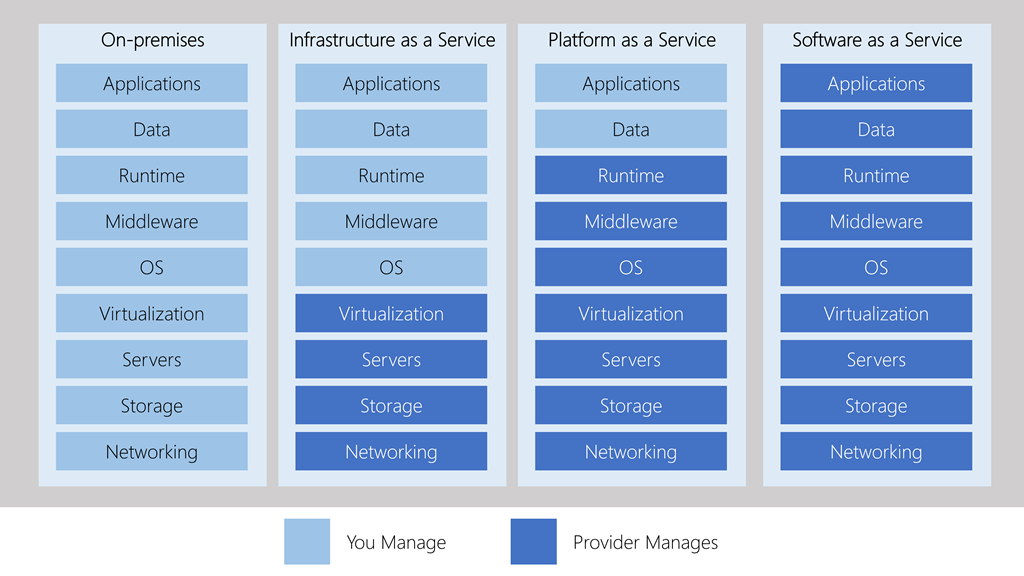
\includegraphics[width=15cm]{5-layer-diagram}
\end{center}

\end{document}
